\documentclass[12pt]{article}
\textwidth=17cm \oddsidemargin=-0.5cm \evensidemargin=-0.5cm
\textheight=23.7cm \topmargin=-1.4cm
\pagestyle{plain}

\usepackage{color}
\usepackage{amssymb, amsmath, amsfonts,mathrsfs,amsthm}
\usepackage{moreverb}
\usepackage{graphicx} %includegraphics[scale=#]{filename}
\usepackage{subcaption}
\usepackage{float}
\usepackage{pdfsync}
\usepackage{hyperref}  
\hypersetup{colorlinks=true}    
\usepackage{bbm}
\usepackage{tcolorbox}
\usepackage[export]{adjustbox}

\def\C{\mathbb{C}}
\def\N{\mathbb{N}}
\def\Q{\mathbb{Q}}
\def\R{\mathbb{R}}
\def\Z{\mathbb{Z}}


\begin{document}
	\title{MAT 128B: Project I}
	
	\author{Joel Aguayo, Joel Barnett, and Doug Kubota }
	\maketitle
	
	\section{Introduction}
	\noindent This project explores Julia and Mandelbrot sets. Group members Aguayo, Barnett and Kubota jointly worked on each section.
	
	Given the function $\phi(z)=z^2+c$, where $c\in \C$ is some costant, we consider the problem of finding the fixed points of $\phi(z)$ using an iterative method. The usual process starts with some $z_0\in \C$ and uses the relation $z_{k+1}=\phi(z_k)$ to generate a sequence $\{z_n\}$ which may, or may not, converge to a fixed point of $\phi(z)$, depending on the choice of $z_0$. \\
	\newline
	Julia sets study the set of initial points which generate a sequence that remains bounded. That is, we define the filled Julia set defined by 
	$\{z\in \C: \text{the sequence } z_{k+1}=\phi(z_k), \text{ with initial value } z_0=z, \text{ remains bounded}\}$, and define the Julia set to be the boundary of the filled Julia set.
	\section{Julia Sets}
	
	\subsection{Filled Julia Sets on the Unit Disc}
		We start with the simplest case: $\phi(z)=z^2$, which has two fixed points $u=1$ and $v=0$. Clearly, if $|z_0| \leq 1$, the sequence will converge because $|z_1|=|\phi(z_0)| = |(z_0)^2| \leq 1$, which implies $|z_2|\leq 1$ and so forth. Also, it is clear that if $|z_0|>1$, the sequence will diverge, because the modulus of the following terms will continue to grow. Thus, the filled Julia set for $\phi(z)$ is the unit disc $D^2=\{z: |z|\leq 1\}$, and the Julia set is the boundary of this disc. 
		
	Below is a plot of the set, which was generated with the MATLAB code provided in section \ref{code}.\\
					
				
		
			\begin{center}
			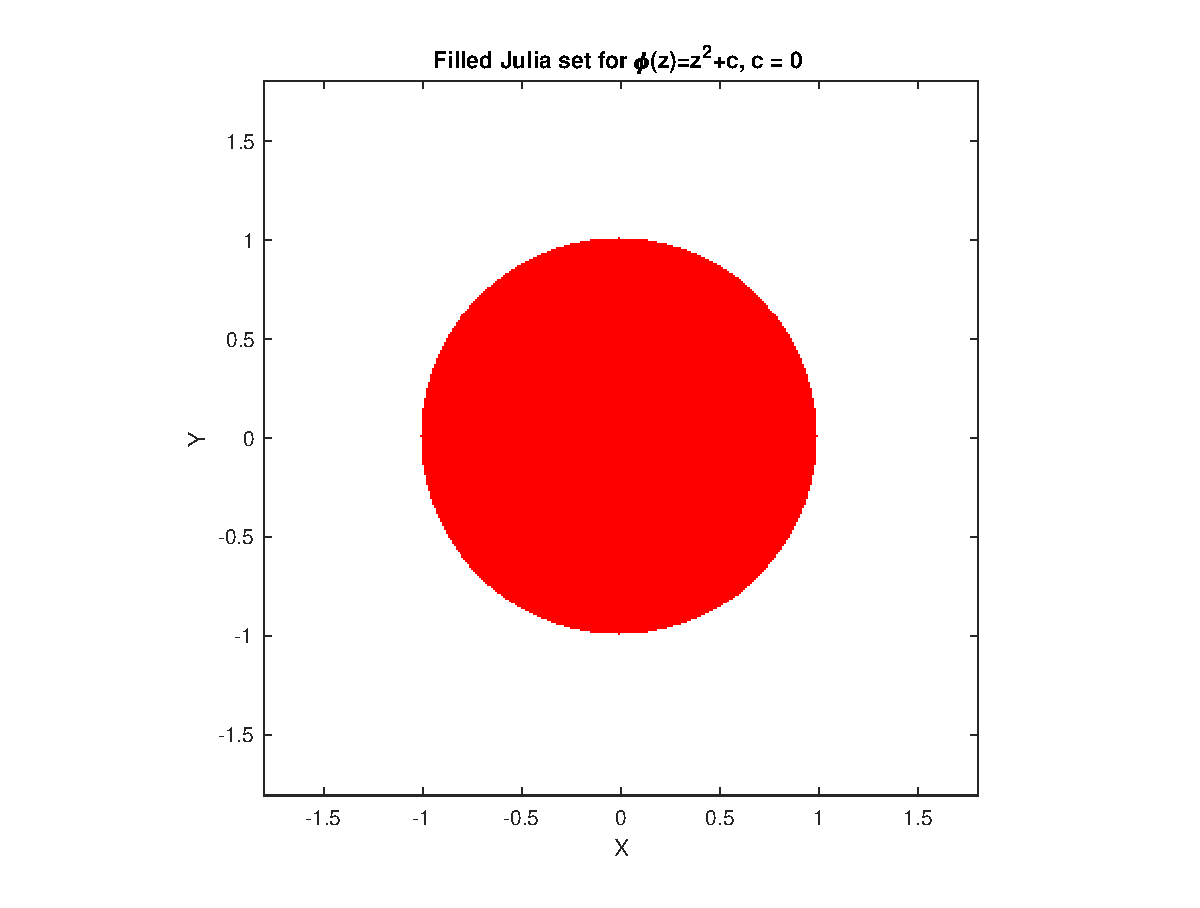
\includegraphics[width=0.5\linewidth]{JSC1}
			\end{center}
	
\subsection{Various Julia Sets} \label{prob2}	
	
	We also graph the Julia set for the function $\phi(z)=z^2+c$, for $c=-1.25,$ $0.36+0.1i,$ $-0.123+0.745i$ and display their graph's below. Note that the code we use to generate these filled Julia sets checks the magnitude of the sequence elements determined by $z_n=\phi(z_{n-1})$. If $|z_n|>2$ for some $n\in \N$, we assume that the sequence is diverging. The algorithm checks all $z_0 \in [-2,2] \times [-2,2]$ region in the complex plane (spaced 0.01 units apart) and plots those which lead to bounded sequences for $z_n$ as red pixels, and those that diverge as white pixels. \\


	
		
	%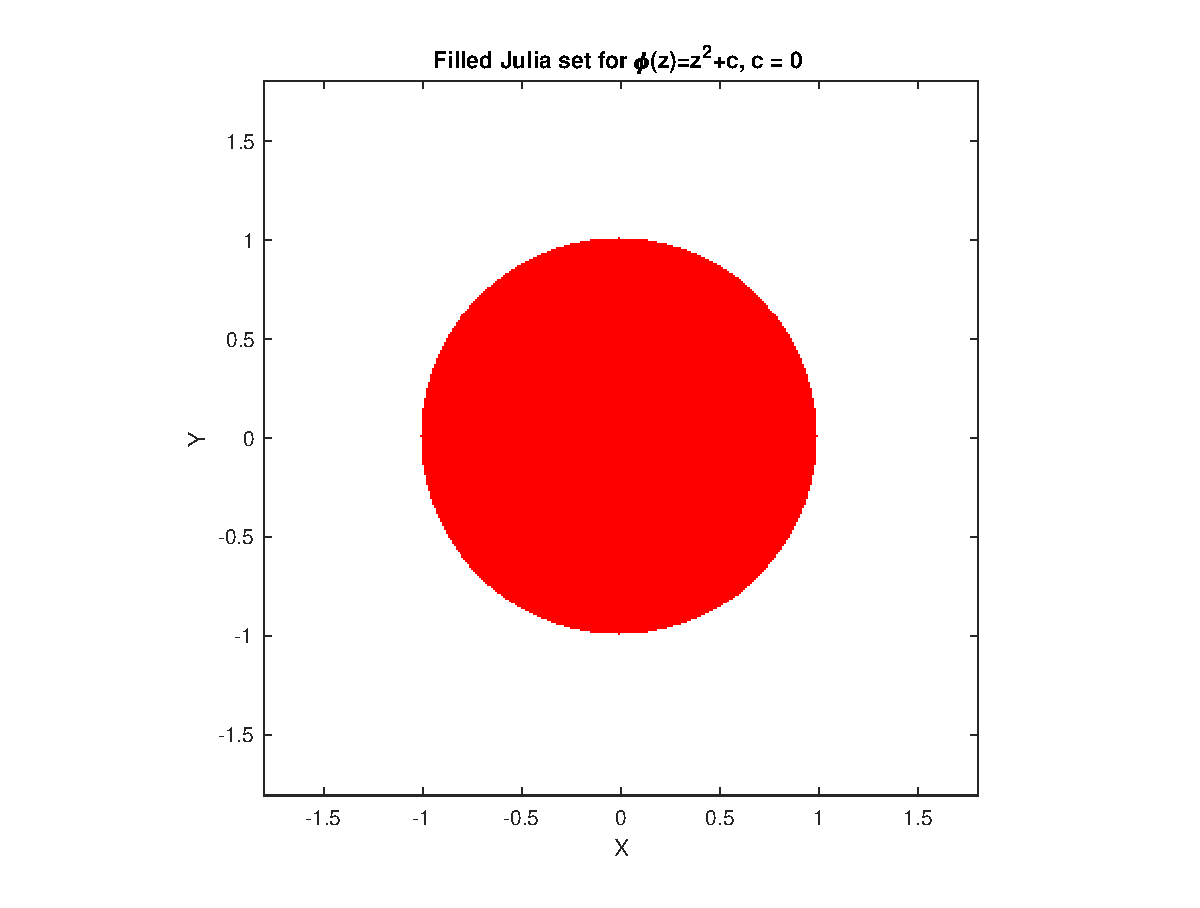
\includegraphics[width=0.49\linewidth]{JSC1.eps}
	\noindent 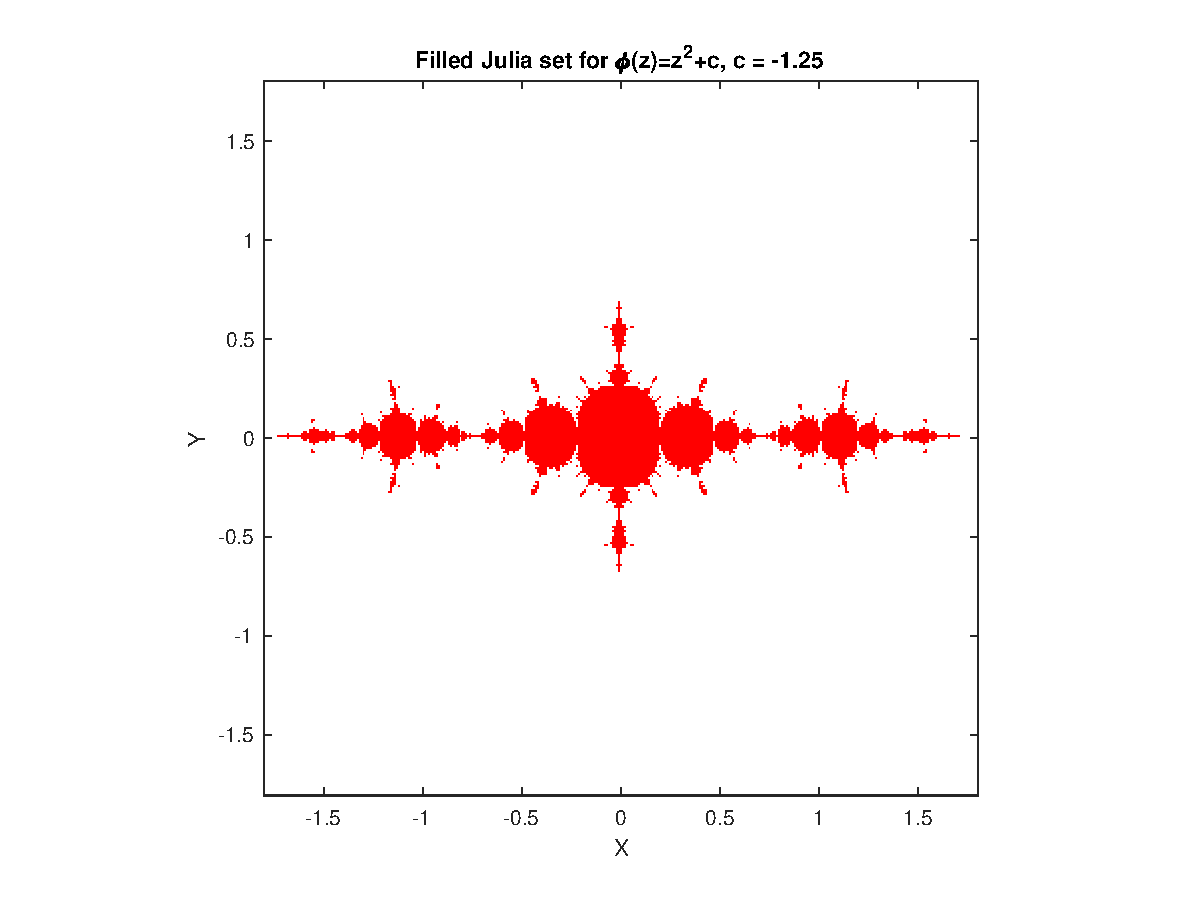
\includegraphics[width=0.49\linewidth]{JSC2.eps}
	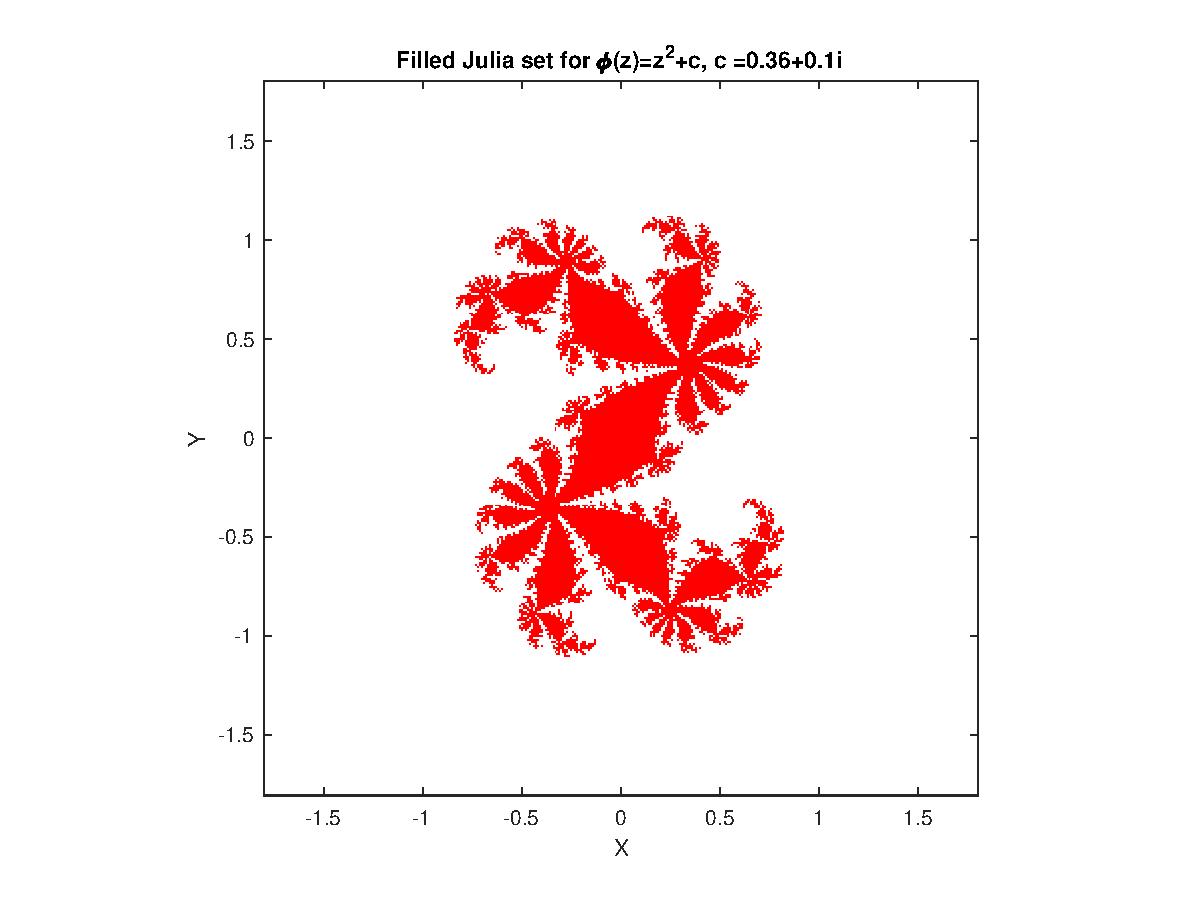
\includegraphics[width=0.49\linewidth]{JSC3.eps}
	\begin{center}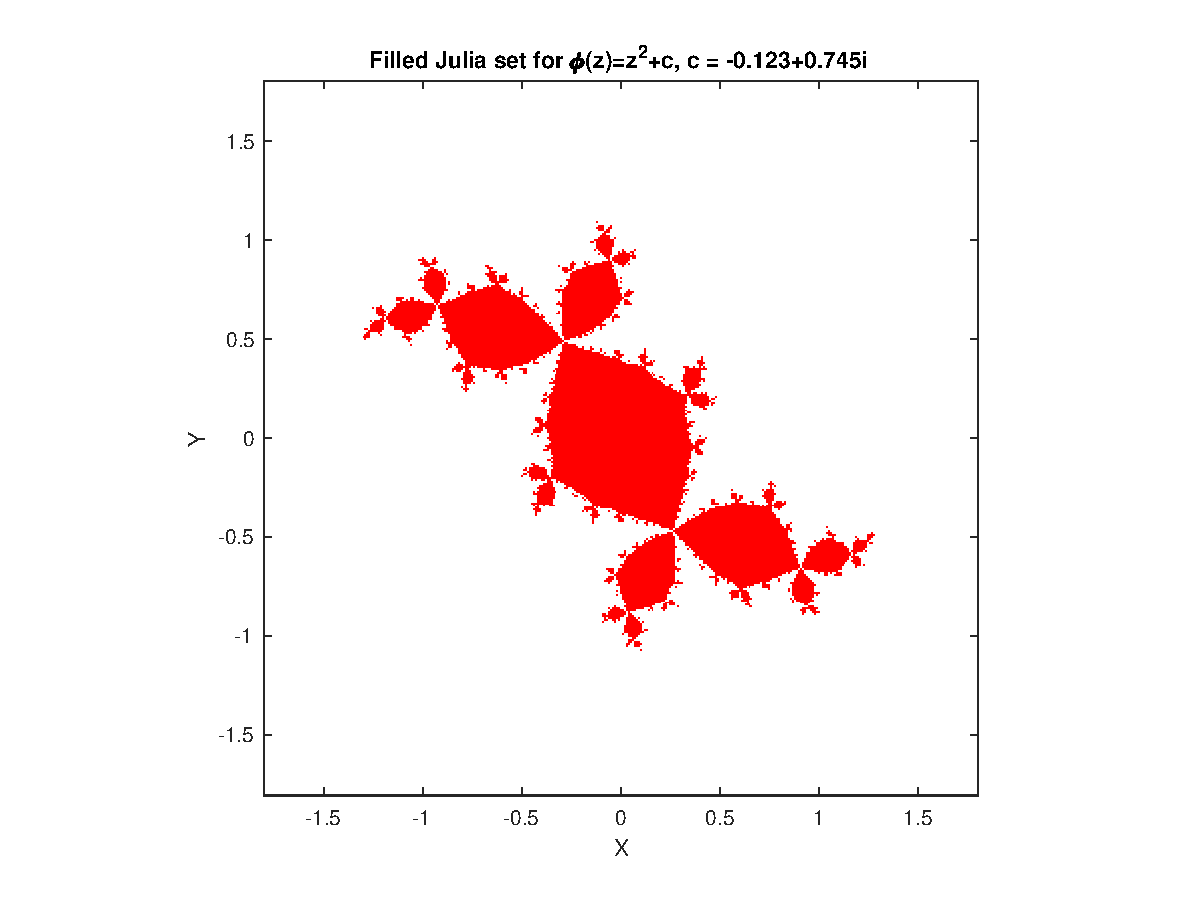
\includegraphics[width=0.49\linewidth]{JSC4.eps}\end{center}
	


\subsection{Boundaries of Filled Julia Sets}\label{prob3}
	We also can form the Julia set by plotting the boundary of the filled Julia sets from section \ref{prob2}. Boundary points are found by noticing that if $\phi(z)=z^2+c$, then $z= \pm \sqrt{\phi(z)-c}$. So, if $z_k = \phi(z_{k-1})$ we get that $z_k= \pm \sqrt{\phi(z_k)-c}=\pm \sqrt{z_{k+1}-c}$, which provides an iterative method to move backwards in the sequences used to generate filled Julia sets. See \ref{JS} for the sample code which generates the boundaries of the filled Julia sets from \ref{prob2}, as shown below.\\
	    
	
	\noindent 
	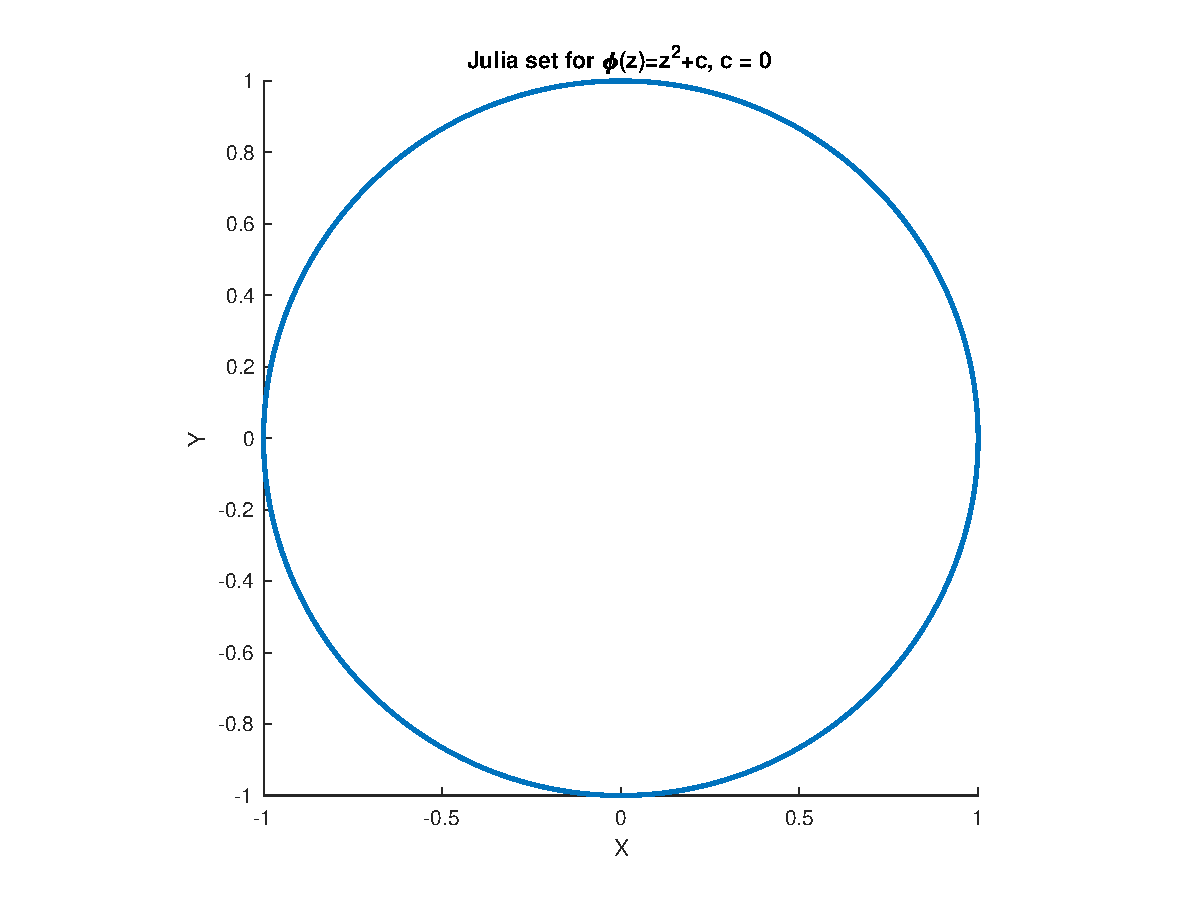
\includegraphics[width=0.49\linewidth]{juliaBound_1.eps}
	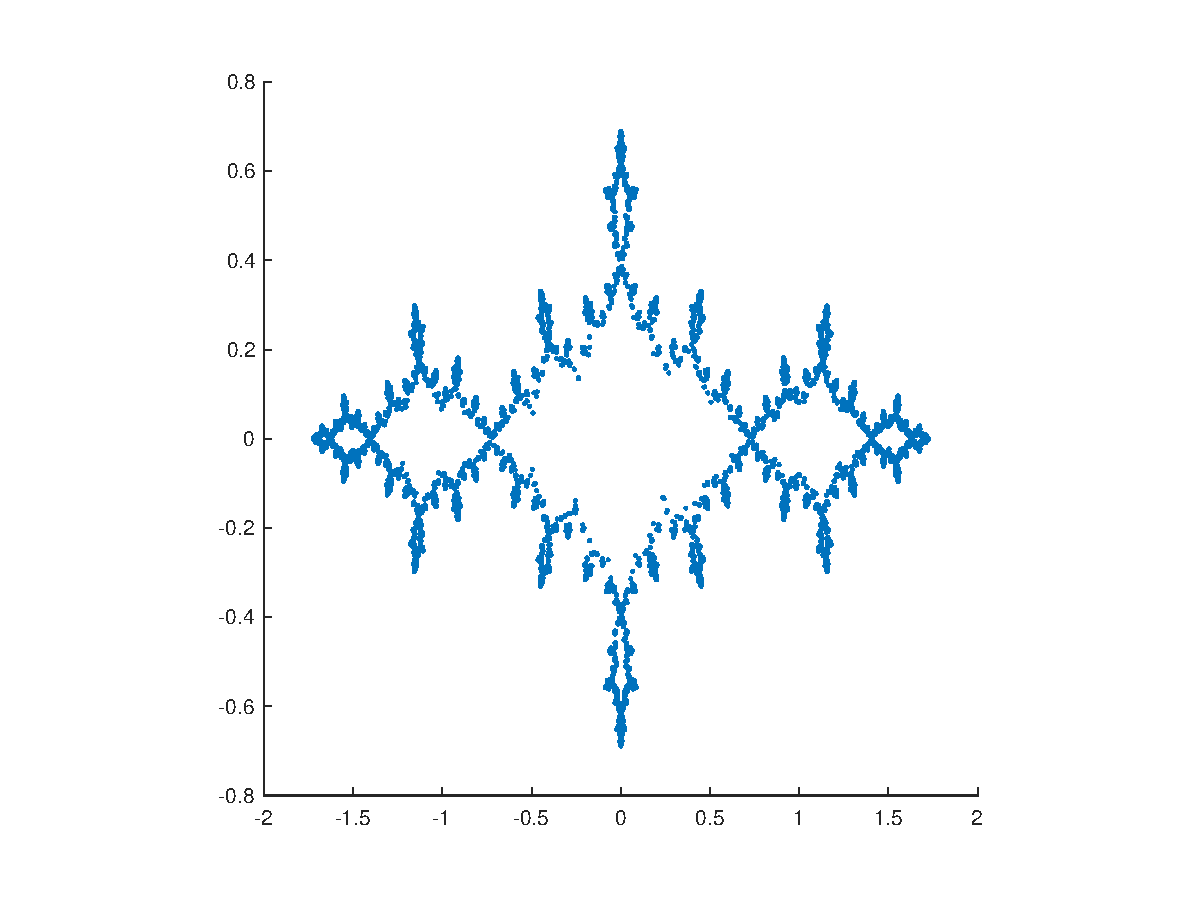
\includegraphics[width=0.49\linewidth]{juliaBound_2.eps}\\
	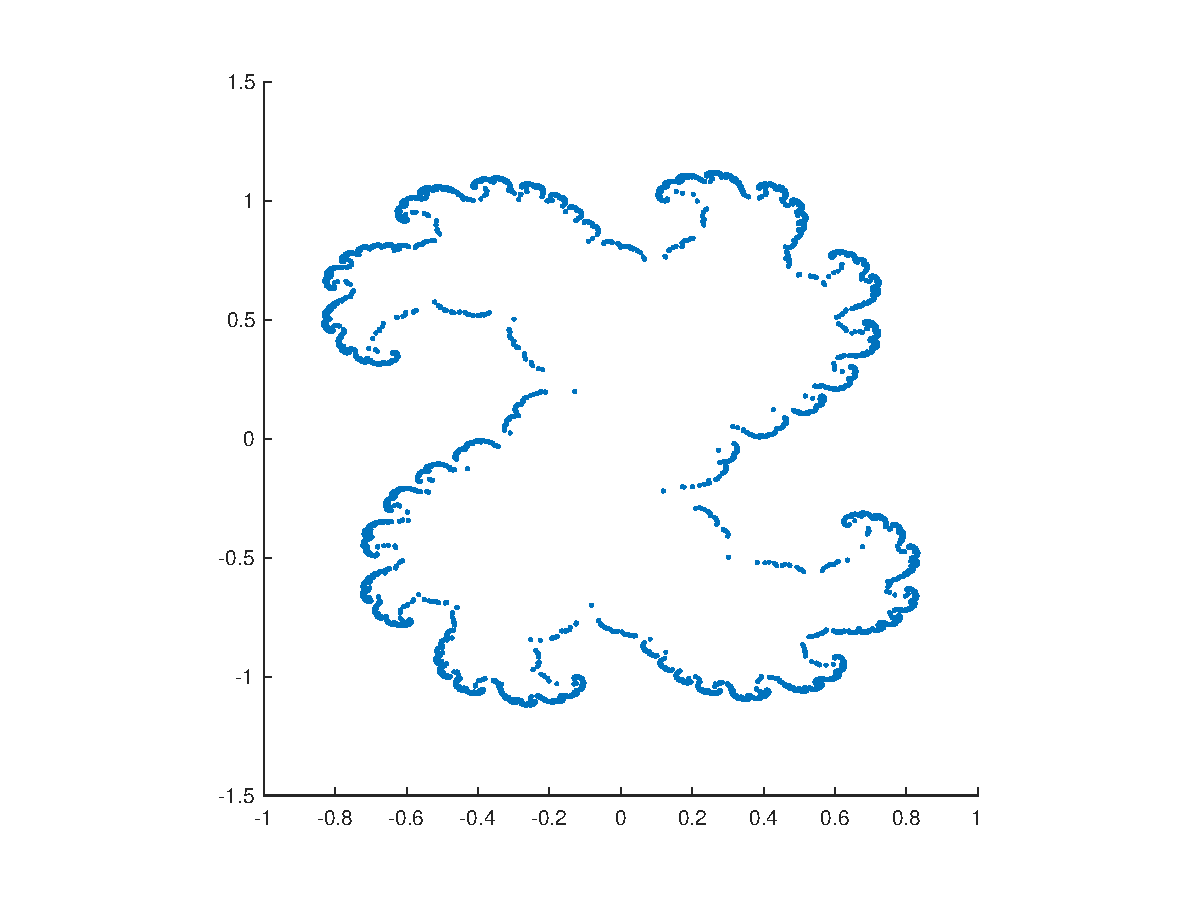
\includegraphics[width=0.49\linewidth]{juliaBound_3.eps}
	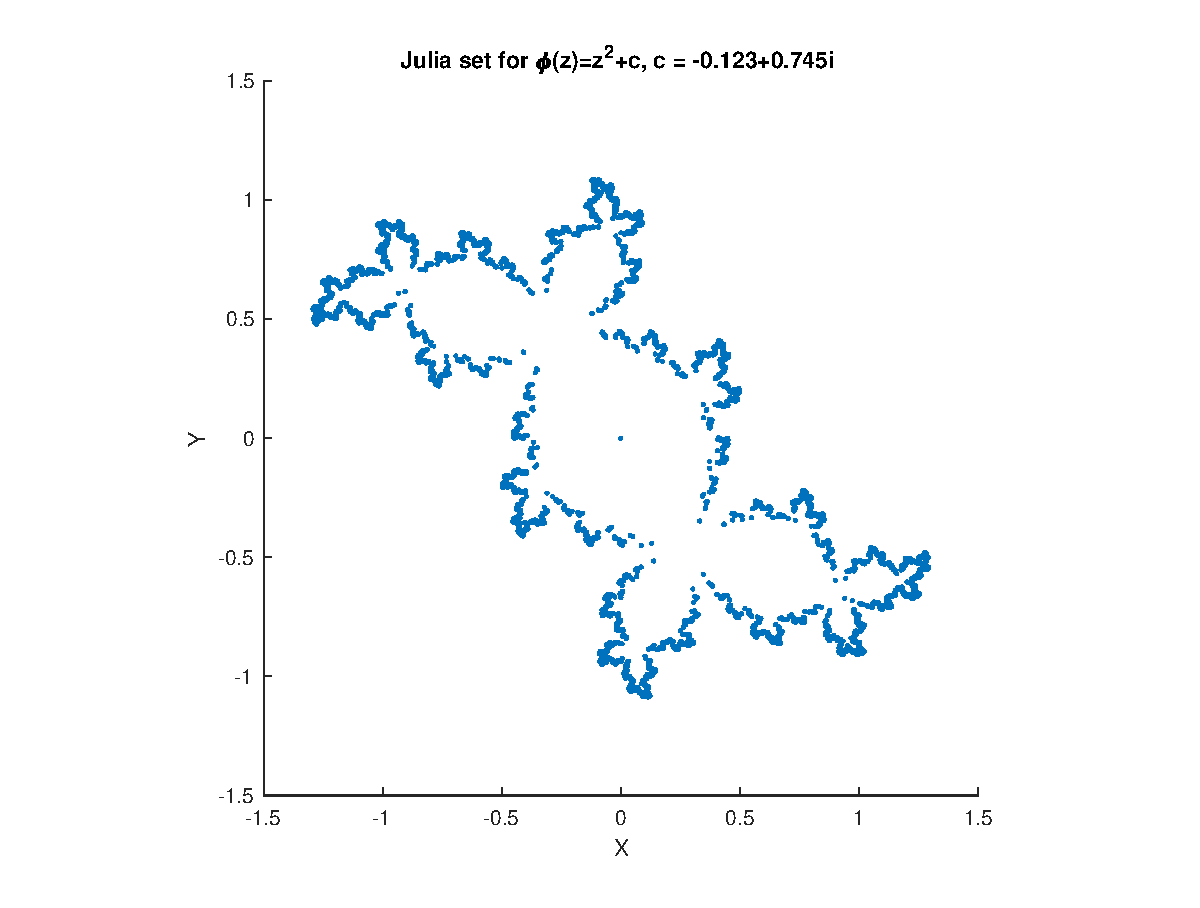
\includegraphics[width=0.49\linewidth]{juliaBound_4.eps}

\section{Computing Fractal Dimentions}
The fractal dimension is used to describe fractals. Fractals generally have a non-integer dimension, so the fractal dimension value is used as an index to describe how the fractal’s pattern changes while it is scaled. It can be used to measure the degree of roughness of a shape. If we place our shape on a grid, its “length” can be viewed as the total amount of boxes that overlap the shape. As we increase or decrease the size of our shape (keeping the grid the same), the number of boxes touching the shape will increase or decrease respectively. The “length” which has now increased or decreased, has a scaling factor. This scaling factor raised to the value of the fractal dimension is used to compute its new size. Simple math can be used to compute the fractal dimension as well. This is easily seen for objects of known dimension.\\
For example, a line is of dimension one, and if we let $L=length$ and scale $L$ by $M$ to give a new line with length $N$, we expect the length to scale linearly to $N=LM$. Thus, our dimension is the $D$ such that $M^D*L=N$, which is easily seen to be $D=1$. If we use a 2D object, such as a disc, and scale a disc of area $A$ by $M$ in every dimension, we expect the final area, $N$, to be $M^2*A$. Thus, our dimension is $D=2$.\\ 

In general, we let $M$ be our scaling factor and $N$ be our scaled "object". Our fractal dimension is $D$ such that:  \\
$M^{D} = N \Rightarrow D =$ log$_{M}(N)$\\
\newline
We implement the reticular cell counting and differential box counting algorithms to compute the fractal dimensions, and test it on the unit circle fractal below. Note that we expect a dimension of $1$ for the unit circle since the length of the circumference is proportional to the radius, so scaling the radius by $M$ will only increase to the length $N=ML$, so the dimension is $D=1$. Code for these is provided in section \ref{dim}.

	\begin{verbatim}
	>> Project1_4
	
	fd =
	
	0.9462
	\end{verbatim}



\section{Orbits}

While the filled Julia set studies whether or not the initial starting point $z_0$ will produce a bounded or converging sequence $\{z_n\}$ under $\phi$, it can be worthwhile to investigate the sequence $\{z_n\}$ itself. We do this by looking at the orbit of a particular $z_0$, where the orbit (denoted by $orb(z_0)$) is given by the set of all elements in the sequence $\{z_n\}$ generated by $\phi$. 
	
\subsection{Connectedness of the Filled Julia Set}
The complex nature of Julia Sets brings up the question of whether or not the filled Julia set is connected (in the topological sense). Surprisingly, there is a simple necessary and sufficient condition for connectedness. Julia and Fatou showed that the filled Julia set for $\phi(z)=z^s+c$ is connected if, and only if, $0$ is in the filled Julia set. Using this condidtion, we develop an algorithm that checks whether or not the $orb(0)$ for a particular $\phi$ is bounded. Boundedness implies that $0$ is in the filled Julia set for $\phi$, so the set is connected. From an algorithmic standpoint, it is difficult to determine with complete certainty that an orbit is bounded since the orbit may remain bounded for many terms and then diverge, or it might grow quickly and then cycle and remain bounded. So, our algorithm checks the first 1000 terms of $orb(0)$ and if the terms remain bounded by 100, we conclude that $orb(0)$ is bounded. Below is the MATLAB output from our algorithm (see section \ref{orbit}) which checks the boundedness of $orb(0)$
\begin{verbatim}
>> Orb_0(0)
The sequence orb(0) converges to a root; thus, the filled Julia set is connected 
Orb(0) remained bounded for 1000 iterations. We assume the filled set is connected 
>> Orb_0(-1.25)
Orb(0) remained bounded for 1000 iterations. We assume the filled Julia set is connected 
>> Orb_0(0.36+0.1*1i)
Orb(0) remained bounded for 1000 iterations. We assume the filled Julia set is connected 
>> Orb_0(-0.123+745*1i)
The orb(0) is unbounded, so the filled Julia set is not connected 
\end{verbatim}
   
\subsection{Coloring Divergent Orbits}
We can also study how fast an orbit diverges. We do this by computing the sequence $z_n$ generated by $phi$. When $|z_k|>1000$ for some $k$, we assign a color to the matrix element corresponding the location of $z_k$ in the complex plane. For colors that diverge at similar points in the sequence (I.e for similar $k$ values), the color is similar. Printing this gives a good idea at how fast points near the boundary of the filled Julia set are diverging. Below is the algorithm, and a sample output for $\phi(z)=z^2+0.36+0.1\cdot i$ and $\phi(z)=z^2-0.123+0.745i$.\\ 
   \newline
   \noindent \includegraphics [width=0.49\linewidth]{ColorOrbit_3.eps}
   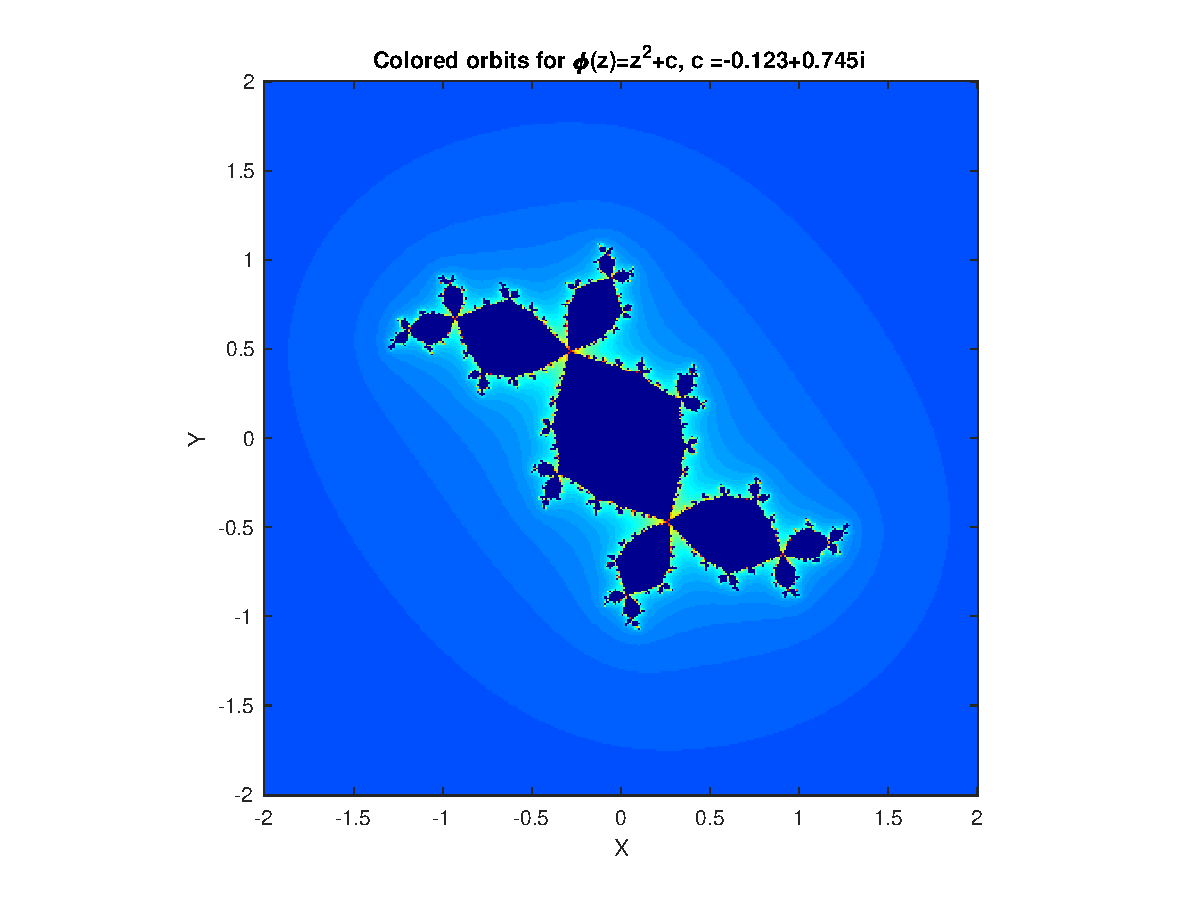
\includegraphics[width=0.49\linewidth]{ColorOrbit_4.eps}
   
    
\section{A Newton's Method Approach}
Rather than only look at $\phi(z)=z^2+c$ as is done in Julia sets, we can also use Newton's method to find the roots of a function of the form $f(z)=z^n+c$. We can then observe which $z_0$ will produce a sequence induced by Newton's method which converges to one of the $n$-roots of $f$. Further, by coloring each of these $z_0$ a different color, we get fractal akin to the Julia set. Below is a sample for the function $f(z)=z^3+1$, where the red, green, and blue sections represent starting points that converge to $1$, $e^{\pi/3 i}$, and $e{-\pi/3i}$, respectively. The algorithm which produces this is provided in section \ref{NM}.

\begin{center}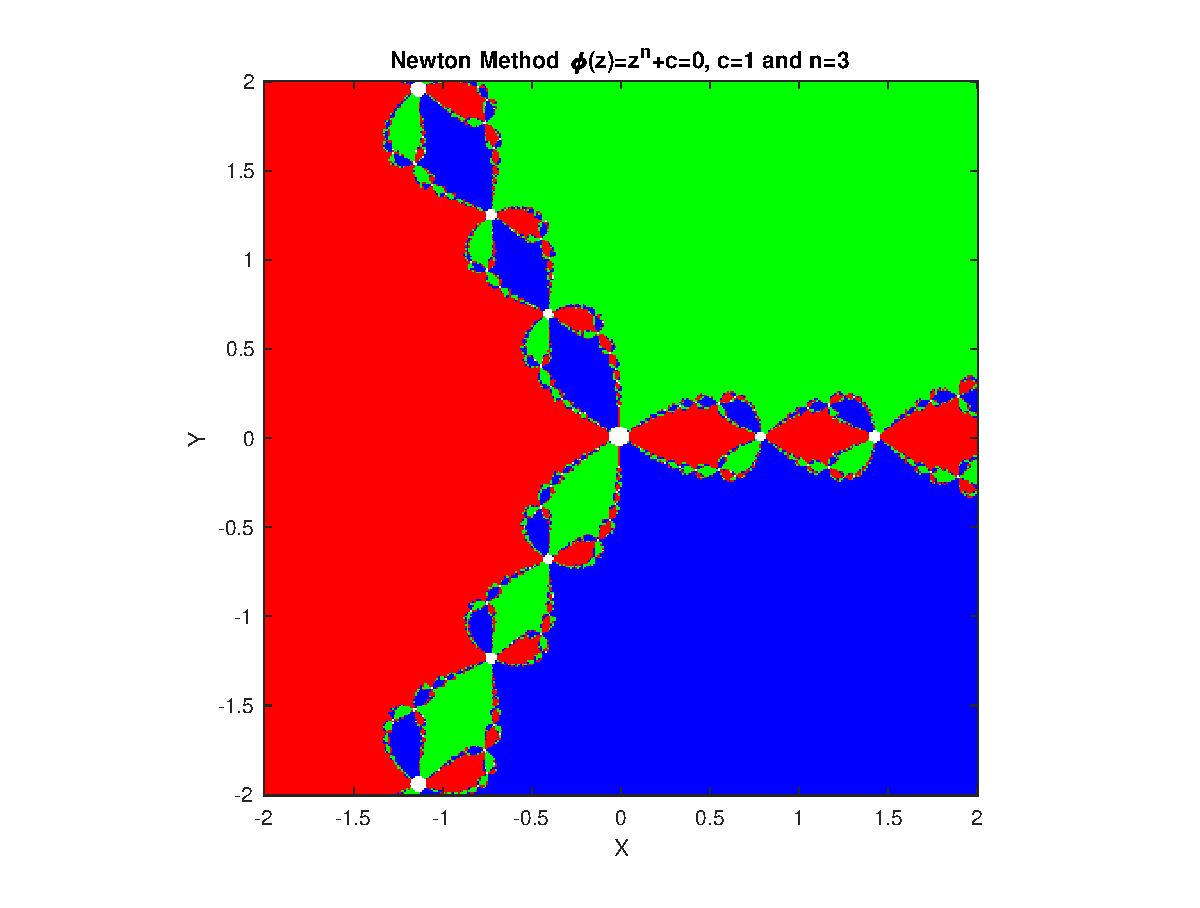
\includegraphics[width=0.7\linewidth]{NMJS.eps} \end{center}

\section{Mandelbrot Sets}
As opposed to Julia sets which study the boundedness of the sequence $\{z_n\}$ for fixed $\phi$, we can choose to check whether the filled Julia set is connected for varying $\phi$ by changing the constant $c$ values. That is, given $c\in \C$, define $\phi(z)=z^2+c$, and check $orb(0)$ for $phi$. Studying which $c$ produces bounded zero-orbits gives the Mandelbrot set. Below is an image of the Mandelbrot set and an algorithm which computes the set is provided in \ref{mandelbrot}. \\
 
 \begin{center} 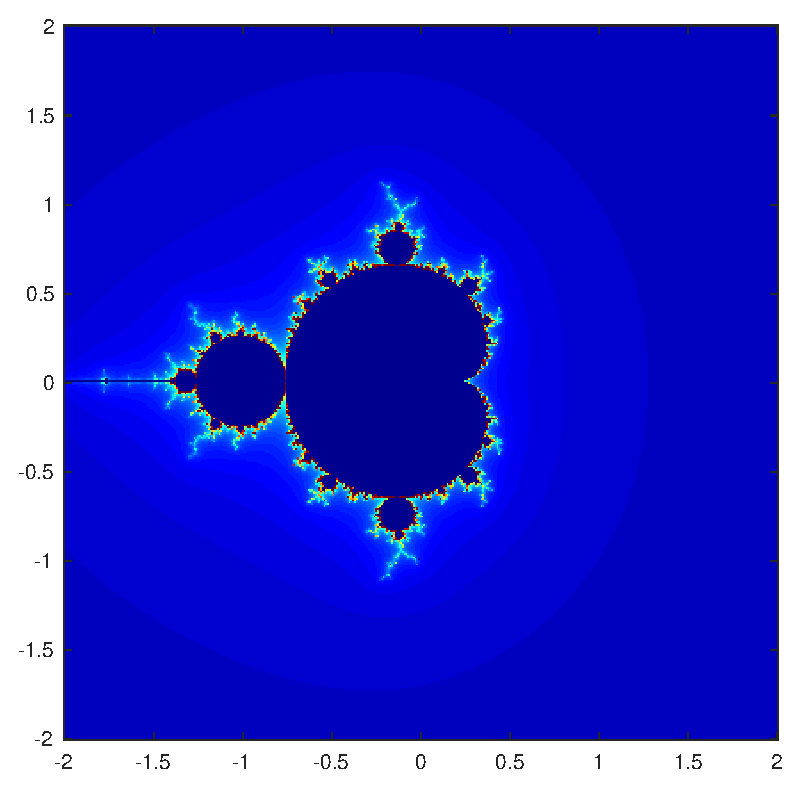
\includegraphics [width=0.5\linewidth]{Mandelbrot_01.eps} \end{center}
 
 




\section{MATLAB Code} \label{code}
	\subsection{Julia Sets} \label{JS}
\noindent	Below is the code which prints the filled Julia set:\\
	
	\begin{verbatim}
	% plots Julia set for z^2 + c
	c= 0.36 +0.1*1i ;   % Define the constant c
	phi = @(z) z^2 + c; % Define the function whose fixed points we seek.
	fixpt1 = (1 + sqrt(1-4*c))/2;
	fixpt2 = (1 - sqrt(1-4*c))/2;
	
	colormap([1 0 0; 1 1 1]);     % Points numbered 1 (inside) will be colored red;
	%   those numbered 2 (outside) will be colored white.
	M = 2*ones(361,361);          % Initialize array of point colors to 2 (white).
	
	for j=1:361                  % Try initial values with imaginary parts between
	y = -1.8+ (j-1)*.01;        %   -1.8 and 1.8
	for i=1:361                % and with real parts between
	x = -1.8 + (i-1)*.01;     %   -1.8 and 1.8.
	z = x + 1i*y;             
	zk = z;
	iflag1 = 0;               % iflag1 and iflag2 count the number of iterations
	iflag2 = 0;               %   when a root is within 1.e-6 of a fixed point;
	kount = 0;                % kount is the total number of iterations.
	
	while kount < 100 & abs(zk) < 2 & iflag1 < 5 & iflag2 < 5
	kount = kount+1;
	zk = phi(zk);           % This is the fixed point iteration.
	err1 = abs(zk-fixpt1);  % Test for convergence to fixpt1.
	if err1 < 1.e-6
	iflag1 = iflag1 + 1;
	else
	iflag1 = 0;
	end
	err2 = abs(zk-fixpt2);  % Test for convergence to fixpt2.
	if err2 < 1.e-6,
	iflag2 = iflag2 + 1;
	else
	iflag2 = 0;
	end;
	end;
	if iflag1 >= 5 | iflag2 >= 5 | kount >= 100   % If orbit is bounded, set this
	M(j,i) = 1;                                  %   point color to 1 (red).
	end
	end
	end
	
	image([-1.8 1.8],[-1.8 1.8],M),  % This plots the results.
	title('Filled Julia set for \phi(z)=z^2+c, c =0.36+0.1i')
	xlabel('X')
	ylabel('Y')
	pbaspect([1 1 1]); %keeps the x/y ratio even
	axis xy            % If you don't do this, vertical axis is inverted.
	\end{verbatim}
	
	\noindent Below is the code which prints the boundary of a filled Julia set: \\

	\begin{verbatim}
	% plots Julia set for z^2 +c
	c= 0.36+.1*1i;   % Define the function whose fixed points we seek.
	
	phiInv= @(z) sqrt(z-c); %this is the inverse iteration of a point
	
	%these holds the real values of the points on the boundary of the filled Julia sets
	Rphi=[200^2];
	Iphi=[200^2];
	arraycount=0;
	
	for j=1:201                  % Try initial values with imaginary parts between
	y = -1+ (j-1)*.01;        %   -1 and 1
	for i=1:201                % and with real parts between
	x = -1 + (i-1)*.01;     %   -1 and 1.
	arraycount=arraycount+1; %increment the Iphi/Rphi arraycount
	zk=x+y*1i;      %set zk to the point in the [-1,1]x[-1,1] region
	kcount=0;       %counter for reverse iteration
	
	%run reverse iteration untill it reaches boundary, kick out if it
	%diverges
	while kcount < 100 && abs(zk) < 2
	n=randi(2,1);
	y=imag(zk-c);
	kcount = kcount+1;
	zk=(-1)^n*phiInv(zk);
	
	end
	%zk is now on the boundary, so set the real and imaginary arrays to its
	%value there
	if abs(zk)<2
	Rphi(arraycount)=real(zk);
	Iphi(arraycount)=imag(zk);
	end
	end
	end
	%plot the Rphi vs Iphi
	scatter(Rphi,Iphi,'.')
	title('Julia set for \phi(z)=z^2+c, c =0.36+0.1i')
	xlabel('X')
	ylabel('Y')
	pbaspect([1 1 1]);  %keep aspect ration square
		
	\end{verbatim}

\subsection{Fractal Dimensions}\label{dim}
Below is the algorithm for the reticular cell counting method.

	\begin{verbatim}
	% PART 4
	% FRACTAL DIMENSION
	
	% RETICULAR CELL COUNTING METHOD
	% STEP 1
	% Convert image to grayscale image
	im = imread('discBoundary.jpg');
	image(im);
	axis image;
	im = im(1:800,201:1000,3);
	bi = (im<200);
	
	imagesc(bi);
	colormap gray;
	axis image;
	
	% STEP 2
	% Determine dimensions of image
	[row,col] = size(bi);
	
	N = zeros(1,3);     % Total number of boxes that contain at least one gray level
	% intensity surface.
	L = [3 2 5];        % Dimension of grids
	
	% STEP 3
	% Count number of boxes containing non white entries
	N(1,1) = grayCount(row,col,L(1,1),bi);
	N(1,2) = grayCount(row,col,L(1,2),bi);
	N(1,3) = grayCount(row,col,L(1,3),bi);
	
	% STEP 4
	% Use least squares method to determine value of D
	Nl = log(N);
	Ll = log(L);
	
	p = polyfit(log10(L),log10(N),1);
	fd=-p(1)
	
	
	function [ N ] = grayCount(row, col, L, imgray)
	%UNTITLED2 Summary of this function goes here
	%   Detailed explanation goes here
	N=0;
	for i=1:L:row                               % Counts across rows by L
	for j=1:L:col                           % Counts across columns by L
	% Searches for a non white pixel in the grid.
	if (i+L < row) && (j+L<col)
	for k=0:L                           % Counts from row i to i+L
	for m=0:L                       % Counts from frow j to j+L
	if imgray(i+k,j+m)==1       % White in matlab for grayscale
	% is equal to 3.
	% If the pixel is not white,
	% then increments the number of
	% nonwhite boxes by 1. Then
	% moves onto the next grid.
	N = N+1;
	k=L+1;                  % The break term exits the for
	% m=0:L loop. Setting k=L+1
	% exits the for k=0:L loop
	% forcing it to move onto the
	% next loop.
	break
	else
	N=N;
	end
	end
	end
	end
	end
	end
	
	
	\end{verbatim}	
	
	
	
\subsection{Orbits}\label{orbit}
	This is the function for computing the $orb(0)$ implemented in MATLAB:
	\begin{verbatim}
	function Orb_0(const)
	% Checks if 0 is in the filled Julia Set for a given \phi(z)=z^2+c
	% by computing the orbit of 0.
	
	%Define the c and initial z_0 (for orb(0), use z0=0;
	c=const;
	z0=0;
	
	%Define the functions and fixed points.
	phi = @(z) z^2 + c;
	fixpt1 = (1 + sqrt(1-4*c))/2;
	fixpt2 = (1 - sqrt(1-4*c))/2;
	
	
	iflag1 = 0;     % iflag1 and iflag2 count the number of iterations
	iflag2 = 0;     %   when a root is within 1.e-6 of a fixed point;
	kount = 0;      % kount is the total number of iterations.
	zk=z0;          %calculates the orb(z_0).
	
	while kount < 1000 && abs(zk) < 100 && iflag1 < 5 && iflag2 < 5
	kount = kount+1;
	zk = phi(zk);           % This is the fixed point iteration.
	err1 = abs(zk-fixpt1);  % Test for convergence to fixpt1.
	if err1 < 1.e-6
	iflag1 = iflag1 + 1;
	else
	iflag1 = 0;
	end
	err2 = abs(zk-fixpt2);  % Test for convergence to fixpt2.
	if err2 < 1.e-6
	iflag2 = iflag2 + 1;
	else
	iflag2 = 0;
	end
	end
	
	if iflag1 >= 5 || iflag2 >= 5    % If orb(0) converges to a root, 
	fprintf('The sequence orb(0) converges to a root; thus, the filled Julia set is connected \n');% 0 is in the filled julia set
	elseif kount >= 1000 %otherwise, if the orbit remained bounded for large iterations
	fprintf('Orb(0) remained bounded for 1000 iterations. We assume the filled Julia set is connected \n'); 
	else
	fprintf('The orb(0) is unbounded, so the filled Julia set is not connected \n');
	end
	end
	\end{verbatim}
	
	
	
\noindent	Below is the colored orbit algorithm:\\

\begin{verbatim}
% Checks the orbits of z_0 from the region [-2,2]x[-2,2]
% under phi(z)=z^2+c

%Define the c
c=0.36+0.1*1i;

%Define the functions and fixed points.
phi = @(z) z^2 + c;
fxpt1 = (1 + sqrt(1-4*c))/2;
fxpt2 = (1 - sqrt(1-4*c))/2;

colormap jet;
M= zeros(401,401);
for j=1:401                  % Try initial values with imaginary parts between
y = -2+ (j-1)*.01;        %   -2 and 2
for i=1:401                % and with real parts between
x = -2 + (i-1)*.01;     %   -2 and 2.
z = x + 1i*y;
zk = z;

iflag1 = 0;     % iflag1 and iflag2 count the number of iterations
iflag2 = 0;     %   when a root is within 1.e-6 of a fixed point;
kcount = 0;      % kount is the total number of iterations.


while kcount < 1000 && abs(zk) < 100 && iflag1 < 5 && iflag2 < 5
kcount = kcount+1;
zk = phi(zk);           % This is the fixed point iteration.

err1 = abs(zk-fixpt1);  % Test for convergence to fixpt1.
if err1 < 1.e-6
iflag1 = iflag1 + 1;
else
iflag1 = 0;
end

err2 = abs(zk-fixpt2);  % Test for convergence to fixpt2.
if err2 < 1.e-6
iflag2 = iflag2 + 1;
else
iflag2 = 0;
end

end

if abs(zk)>100 %if the orbit diverged, fill in the color map
M(j,i)=kcount; %the color for terms that diverged with similar
%kcounts will have similar color
end
end
end

image([-2 2],[-2 2],M),  % This plots the results.
pbaspect([1 1 1]); %keeps the x/y ratio even
axis xy % prevents inverted xy axis
\end{verbatim}

	\subsection{Newton's Method}\label{NM}
	\begin{verbatim}
	% Forms the julia set using Newton's method iteration for finding roots to
	% z^n+c=0
	
	% define the degree of polynomai
	n=3;
	%Define the c
	c=1;
	
	%Define the functions and fixed points.
	f = @(z) z.^n + c;
	fprime = @(z) n*z^(n-1);
	fixpt1 = 1;
	fixpt2 = exp(pi/3*1i);
	fixpt3= exp(-pi/3*1i);
	
	colormap([1 0 0;0 1 0; 0 0 1; 1 1 1]); %color map with n+1 colors
	M= zeros(401,401);
	for j=1:401                  % Try initial values with imaginary parts between
	y = -2+ (j-1)*.01;        %   -2 and 2
	for i=1:401                % and with real parts between
	x = -2 + (i-1)*.01;     %   -2 and 2.
	z = x + 1i*y;             
	zk = z;
	
	iflag1 = 0;     % iflag1, iflag2, and iflag3 count the number of iterations
	iflag2 = 0;     %   when a root is within 1.e-6 of fixed points 1,2,3;
	iflag3 = 0;
	kcount = 0;      % kount is the total number of iterations.
	
	
	while kcount < 100 && abs(zk) < 100 && iflag1 < 5 && iflag2 < 5 && iflag3<5
	kcount = kcount+1;
	zk = zk-f(zk)/fprime(zk);           % This is the newtons method iteration.
	
	err1 = abs(zk-fixpt1);  % Test for convergence to fixpt1.
	if err1 < 1.e-6
	iflag1 = iflag1 + 1;
	else
	iflag1 = 0;
	end
	
	err2 = abs(zk-fixpt2);  % Test for convergence to fixpt2.
	if err2 < 1.e-6
	iflag2 = iflag2 + 1;
	else
	iflag2 = 0;
	end
	
	err3 = abs(zk-fixpt3);  % Test for convergence to fixpt3.
	if err3 < 1.e-6
	iflag3 = iflag3 + 1;
	else
	iflag3 = 0;
	end
	end
	
	if abs(zk)>100 %if the orbit diverged, fill in the color map
	M(j,i)=4; % to the color white
	
	elseif iflag1>=5
	M(j,i)=1; %if converge to fxp 1, color red
	elseif iflag2>=5
	M(j,i)=2; %if converge to fxp 2, color green
	elseif iflag3 >=5
	M(j,i)=3; %if converge to fxp3, color blue
	end
	end
	end
	
	image([-2 2],[-2 2],M),  % This plots the results.
	title('Newton Method \phi(z)=z^n+c=0, c=1 and n=3')
	xlabel('X')
	ylabel('Y')
	pbaspect([1 1 1]); %keeps the x/y ratio even
	axis xy % prevents inverted xy axis
	
	\end{verbatim}
	
	\subsection{Mandelbrot Code}\label{mandelbrot}
	\begin{verbatim}
	% This program generates the mandelbrot set
	
	%Define the functions and fixed points.
	phi = @(z,c) z^2 + c;
	fixpt1 = @(c) (1 + sqrt(1-4*c))/2;
	fixpt2 = @(c) (1 - sqrt(1-4*c))/2;
	z0=0;       %madelbrot uses z0=0;
	colormap jet;
	
	M= ones(401,401);
	for j=1:401                  % Try initial values with imaginary parts between
	y = -2+ (j-1)*.01;        %   -2 and 2
	for i=1:401                % and with real parts between
	x = -2 + (i-1)*.01;     %   -2 and 2.
	c = x + 1i*y;
	
	
	iflag1 = 0;     % iflag1 and iflag2 count the number of iterations
	iflag2 = 0;     %   when a root is within 1.e-6 of a fixed point;
	kcount = 0;      % kount is the total number of iterations.
	zk=z0;
	%compute the orb(0) for this particular c value
	while kcount < 1000 && abs(zk) < 100 && iflag1 < 10 && iflag2 < 10
	kcount = kcount+1;
	zk = phi(zk,c);           % This is the fixed point iteration.
	
	err1 = abs(zk-fixpt1(c));  % Test for convergence to fixpt1.
	if err1 < 1.e-6
	iflag1 = iflag1 + 1;
	else
	iflag1 = 0;
	end
	
	err2 = abs(zk-fixpt2(c));  % Test for convergence to fixpt2.
	if err2 < 1.e-6
	iflag2 = iflag2 + 1;
	else
	iflag2 = 0;
	end
	
	end
	
	if abs(zk)>100 %if the orbit diverged, fill in the color map
	M(j,i)=kcount; %the color for terms that diverged with similar
	%kcounts will have similar color
	end
	end
	end
	
	image([-2 2],[-2 2],M),  % This plots the results.
	pbaspect([1 1 1]); %keeps the x/y ratio even
	axis xy % prevents inverted xy axis
	\end{verbatim}

	

\subsection{Commit List}\label{commit}
Evidence of GitHub use provided below:\\
\begin{center}\includegraphics[width=0.7\linewidth]{commit} \end{center}
\end{document}